\section{Fluxionnal execution model}

\subsection{Fluxions}

The fluxionnal execution model role is to manage and invoke autonomous execution units.
An execution unit accepts only streams as input and output, that is a continuous and infinite sequence of data contained in messages.
We named this execution unit a fluxion.
That is a function, as in functional programming, only dependent from data streams.
It is composed of a unique name, a processing function, and a memory context during its execution.

Messages are composed of the name of the recipient fluxion, a body, and are carried by a messaging system.
% They represent both the invocation signal, and the data needed for this invocation
After processing a message, the fluxion modify its context, and then terminate its execution by sending a message on its output stream.
Each fluxion sends back a unique message to one or many recipient.
The fluxion's execution context is defined as the set of state variables whose the fluxion depends on, between two rounds of execution.

The fluxions make up a chain of processing binded by data streams.
All these chains make up a directed graph, managed by the messaging system.

\subsection{Messaging system}

The messaging system is the core of our fluxionnal execution model.
It carries messages along stream, and invokes fluxion at a message reception.

It is build around a message queue.
Each message is processed one after another by invocation of the recipient fluxion.
Using a message queue allows to execute multiple processing chain fairly and concurrently, without difference in scheduling local messages, or network messages.
The life cycle of a fluxionnal application is pictured on figure \ref{fig:MesSys}.

\begin{figure}[h!]
  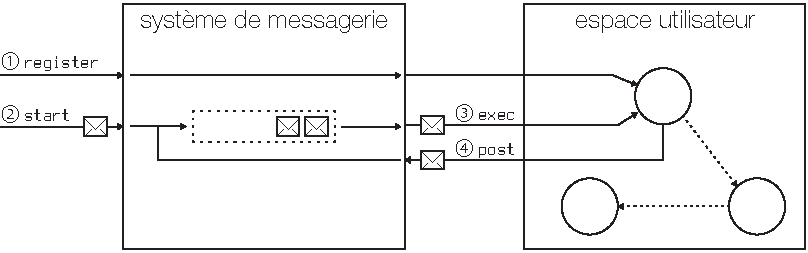
\includegraphics[width=\linewidth]{schema-message.pdf}
  \caption{Messaging system details}
  \label{fig:MesSys}
\end{figure}

The messaging system needs every fluxion to be registered.
This registration match a processing function with a unique name and an initial execution context.
The messaging system carries messages streams based on the names of the recipients fluxions.
That's why two fluxions with the same name would lead the system in a conflicting situation.
The registration is done using the function \texttt{register(<nom>, <fn>, <context>)}, step \circled{1} on figure \ref{fig:MesSys}.
% A fluxion can dynamically register other fluxions

To trigger a fluxions chain, a first \texttt{start(<msg>)} message is sent, step \circled{2}.
This function pushes a first message in the queue.
Immediately, the system dequeues this message to invoke the recipient processing function, step \circled{3} and \circled{4}.
The message resulting of this invocation is then enqueued, step \circled{5} and \circled{6}.
The system loops through steps \circled{3} to \circled{4} until the queue is empty.

The algorithm \ref{alg:traitement} and \ref{alg:parcours} precisely describe the behavior of the messaging system after the function \texttt{start} invocation.

\begin{algorithm}
\caption{Message queue processing algorithm}
\label{alg:traitement}
\begin{algorithmic}
\Function{processMsg}{$msg$}
\For{$dest$ \textbf{in} $msg.dest$}
\State $fluxion \gets lookup(dest)$
\State $message \gets$ \Call{exec}{$fluxion, msg.body$} \Comment{\circled{4} \& \circled{5}}
\State \Call{enqueue}{$message$} \Comment{\circled{6}}
\EndFor
\EndFunction
\end{algorithmic}
\end{algorithm}

\begin{algorithm}
\caption{Message queue walking algorithm}
\label{alg:parcours}
\begin{algorithmic}
\Function{loopMessage}{\null}
\While{$msg$ \textbf{presents in} $msgQueue$}
\State $msg \gets$ \Call{dequeue}{\null} \Comment{\circled{3}}
\State \Call{ProcessMsg}{$msg$}
\EndWhile
\EndFunction
\end{algorithmic}
\end{algorithm}

\subsection{External interfaces}

In order to interact with other systems, we define external border interfaces.
As a first approach, our goal is to interface Web architectures, so we need to communicate with a REST\footnote{REST: \textbf{Re}presentational \textbf{S}tate \textbf{T}ransfer \cite{Fielding2002}} client.
We define two components in this interface :

\begin{itemize}
	\item[\textbf{In}]
    receives client connections.
    % This is so the first link in the chain.
    For every incoming connection, it relays a connection identifier to the \textbf{Out} component for the reply.
    It then relays the connection identifier and the request to the first fluxion by calling the \texttt{start} function.
	\item[\textbf{Out}]
    replies the result of the processing chain to the client.
    To receive messages from the processing chain, the component \textbf{Out} is registered in the messaging system under the name \texttt{out}.
    % This is so the last link in the chain.
\end{itemize}

Figure \ref{fig:schemaweb} pictures the specifics elements of the web interface inside the fluxionnal system.
% La figure \ref{fig:schemaweb} illustre les éléments spécifiques de cette interface Web au sein du système fluxionnal illustré par la figure \ref{fig:MesSys}.

\begin{figure}[h!]
	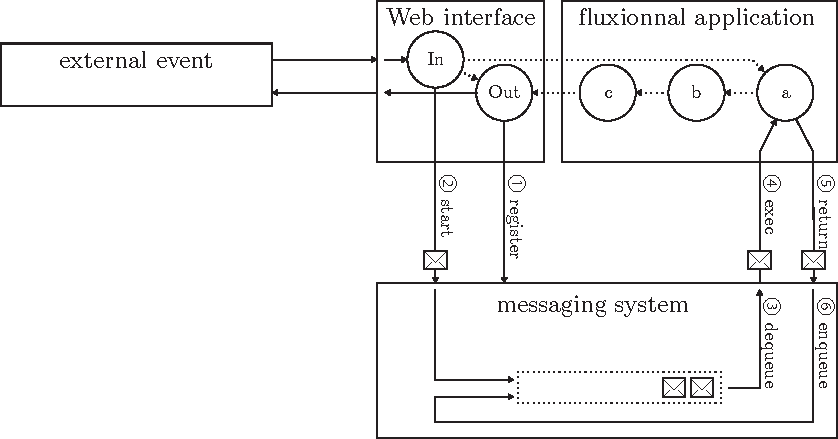
\includegraphics[width=\linewidth]{schema-web.pdf}
	\caption{Fluxionnal application with web interface}
	\label{fig:schemaweb}
\end{figure}

% TODO paragraphe de transition

\subsection{Service example}

In order to picture the fluxionnal execution model, we present an example of a simple visit counting service.
This service counts the number of HTTP connections for each user, and sends him back this number in the HTTP reply.

The initial version of this service could look like listing \ref{lst:classique}.

\begin{code}[Javascript, caption={Initial service},label={lst:classique}]
var app = require('express')();

@\label{lst:classique_count}@var count = {};

@\label{lst:classique_get}\label{lst:classique_replyb}@app.get('/:id', function reply(req, res){
  count[req.params.id] = count[req.params.id]  || 1;
  ++count[req.params.id]
  var visits = count[req.params.id];
  var reply = req.params.id + ' connected ' + visits + ' times.';
@\label{lst:classique_send}@  res.send(reply);
@\label{lst:classique_replye}@});

port = 8080;
app.listen(port);
console.log("Listening port: "+port);
\end{code}

In listing \ref{lst:classique}, three elements are worth noticing.

\begin{itemize}
  \item The \texttt{count} object at line \ref{lst:classique_count} is a persistent memory that stores each user visit count.
  This object is mapped to a fluxion \textit{execution context} in the fluxionnal system.
  \item The \texttt{reply} function, line \ref{lst:classique_replyb} to \ref{lst:classique_replye}, contains the logic we want to express in the fluxionnal processing chain.
  \item The two methods \texttt{get} and \texttt{send}, respectively line \ref{lst:classique_get} and \ref{lst:classique_send}, interface the logic with the external interface.
  The hidden processing chain is : $\texttt{get} \to \texttt{reply} \to \texttt{send}$
\end{itemize}

This minimal service is transformed with our automatic tool into the Figure \ref{fig:fluxions} fluxions chain .

\begin{figure}[h!]
  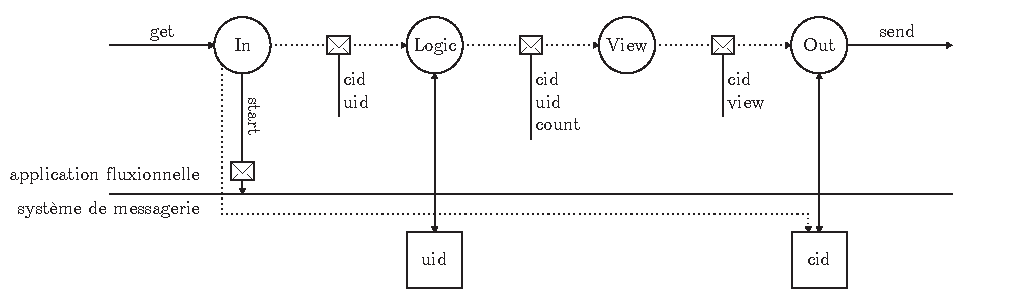
\includegraphics[width=\linewidth]{flux.pdf}
  \caption{Count service fluxions chain}
  \label{fig:fluxions}
\end{figure}

Figure \ref{fig:fluxions}, circles shows registered fluxions.
We show exchanged messages between fluxions and data transmitted from one fluxion to the other. Finally squares stored in the messaging system hold the \textit{execution context} for the logic and \textbf{Out} fluxionx.
When a new \texttt{get} REST message is received at the \textbf{In} end point, a start message triggers the flow.
Concurrently the \textbf{In} fluxion set a \texttt{cid} parameter to the \textbf{Out} fluxion execution context.
This \texttt{cid} is associated to the client connexion the last fluxion may redirect the answer to.
The \texttt{cid} tags the request and is transmitted all the way long through the flow.
Each fluxion propagates the necessary values from one fluxion to the other exclusively within messages.
Horizontal dashed lines shows message virtual transmission between fluxion although they all go through the messaging system.

Listing \ref{lst:fluxionnal} describes this counting service in our fluxionnal language.
Conclusion, this new language brings a stricter segmentation than the initial code, and so allows an additional system to optimize how fluxions are organized on different physical machines according to the cost of the streams and their processing. 

This high level language is not dynamic, and not typed.
You can register fluxion at any time, and the messages can contain any type or composition of types.
\TODO{write a paragraph about the languages characteristics, a reserved subsection might be necessary, but maybe better placed in the next section, about transformation}

\begin{code}[Javascript, caption={Fluxionnal sample},label={lst:fluxionnal}]
use fluxion, web

fluxion logic >> view
  this.uid[msg.uid] = this.uid[msg.uid] + 1 || 1
  msg.count = this.uid[msg.uid]
  return msg

fluxion view >> output
  msg.view = msg.uid + " connected " + msg.count + " times."
  msg.uid = undefined
  msg.count = undefined
  return msg

register logic, {uid: {}}
register view

web.listen
\end{code}

Except from the two interface components, the service is split as follow :
\begin{itemize}
  \item The \texttt{logic} fluxion is the first to receive the client message.
  It contains the whole logic of this simple service.
  A real services would need a more complex chain with logic distributed across multiples fluxions, instead of a single fluxion.
  It increments the count for the received user identifier, push this count inside the message, and relay it the next fluxion.
  \item The \texttt{view} fluxion receive this message, and format as the user will view it, and relay it the output fluxion.
\end{itemize}

We uses this interface to develop web services using the fluxionnal execution model.
We now show the evaluation of this model using different implementation.
